\documentclass[11pt,]{article}
\usepackage{lmodern}
\usepackage{amssymb,amsmath}
\usepackage{ifxetex,ifluatex}
\usepackage{fixltx2e} % provides \textsubscript
\ifnum 0\ifxetex 1\fi\ifluatex 1\fi=0 % if pdftex
  \usepackage[T1]{fontenc}
  \usepackage[utf8]{inputenc}
\else % if luatex or xelatex
  \ifxetex
    \usepackage{mathspec}
  \else
    \usepackage{fontspec}
  \fi
  \defaultfontfeatures{Ligatures=TeX,Scale=MatchLowercase}
\fi
% use upquote if available, for straight quotes in verbatim environments
\IfFileExists{upquote.sty}{\usepackage{upquote}}{}
% use microtype if available
\IfFileExists{microtype.sty}{%
\usepackage{microtype}
\UseMicrotypeSet[protrusion]{basicmath} % disable protrusion for tt fonts
}{}
\usepackage[margin=0.75in]{geometry}
\usepackage{hyperref}
\hypersetup{unicode=true,
            pdftitle={Recipe Book},
            pdfauthor={Brian J. Smith},
            pdfborder={0 0 0},
            breaklinks=true}
\urlstyle{same}  % don't use monospace font for urls
\usepackage{graphicx,grffile}
\makeatletter
\def\maxwidth{\ifdim\Gin@nat@width>\linewidth\linewidth\else\Gin@nat@width\fi}
\def\maxheight{\ifdim\Gin@nat@height>\textheight\textheight\else\Gin@nat@height\fi}
\makeatother
% Scale images if necessary, so that they will not overflow the page
% margins by default, and it is still possible to overwrite the defaults
% using explicit options in \includegraphics[width, height, ...]{}
\setkeys{Gin}{width=\maxwidth,height=\maxheight,keepaspectratio}
\IfFileExists{parskip.sty}{%
\usepackage{parskip}
}{% else
\setlength{\parindent}{0pt}
\setlength{\parskip}{6pt plus 2pt minus 1pt}
}
\setlength{\emergencystretch}{3em}  % prevent overfull lines
\providecommand{\tightlist}{%
  \setlength{\itemsep}{0pt}\setlength{\parskip}{0pt}}
\setcounter{secnumdepth}{0}
% Redefines (sub)paragraphs to behave more like sections
\ifx\paragraph\undefined\else
\let\oldparagraph\paragraph
\renewcommand{\paragraph}[1]{\oldparagraph{#1}\mbox{}}
\fi
\ifx\subparagraph\undefined\else
\let\oldsubparagraph\subparagraph
\renewcommand{\subparagraph}[1]{\oldsubparagraph{#1}\mbox{}}
\fi

%%% Use protect on footnotes to avoid problems with footnotes in titles
\let\rmarkdownfootnote\footnote%
\def\footnote{\protect\rmarkdownfootnote}

%%% Change title format to be more compact
\usepackage{titling}

% Create subtitle command for use in maketitle
\newcommand{\subtitle}[1]{
  \posttitle{
    \begin{center}\large#1\end{center}
    }
}

\setlength{\droptitle}{-2em}

  \title{Recipe Book}
    \pretitle{\vspace{\droptitle}\centering\huge}
  \posttitle{\par}
    \author{Brian J. Smith}
    \preauthor{\centering\large\emph}
  \postauthor{\par}
      \predate{\centering\large\emph}
  \postdate{\par}
    \date{January 19, 2019}

\usepackage{booktabs}
\usepackage{longtable}
\usepackage{array}
\usepackage{multirow}
\usepackage{wrapfig}
\usepackage{float}
\usepackage{colortbl}
\usepackage{pdflscape}
\usepackage{tabu}
\usepackage{threeparttable}
\usepackage{threeparttablex}
\usepackage[normalem]{ulem}
\usepackage{makecell}
\usepackage{xcolor}

\usepackage{graphbox}
\usepackage{mwe}
\usepackage[11pt]{moresize}

\begin{document}
\maketitle

{
\setcounter{tocdepth}{1}
\tableofcontents
}
\break 

\section{Chicken Thighs}\label{chicken-thighs}

\hrule  \vspace{5 mm}

\HUGE Chicken
Thighs\normalsize \hfill \includegraphics[align=c, height=3in]{recipes/Chicken Thighs/chicken_thighs.jpg}

\vspace{5 mm} \hrule 

\subsection{Ingredients}\label{ingredients}

\begin{tabular}{l|l|l}
\hline
Ingredient & Amount & Unit\\
\hline
Olive Oil & 2 & tbsp\\
\hline
Chicken Thighs & 6 & pieces\\
\hline
Salt & to taste & \\
\hline
Pepper & to taste & \\
\hline
Broth & 4 & cups\\
\hline
Water & 2 cups & \\
\hline
Garlic & 5 & cloves\\
\hline
Kale & 1 & bunch\\
\hline
Orzo Pasta & 1 & lb\\
\hline
Parmesan Cheese & to taste & \\
\hline
\end{tabular}

\subsection{Steps}\label{steps}

\begin{enumerate}
\def\labelenumi{\arabic{enumi}.}
\item
  Heat olive oil in a Dutch oven on medium-high heat. Meanwhile, preheat
  the oven to 400°F.
\item
  Season chicken thighs with salt and pepper. Place skin side down in
  the Dutch oven and crisp the skin.
\item
  Chop the garlic coarsely and add to the Dutch oven when you flip the
  chicken. Cook another 3 or 4 minutes on this side.
\item
  Add half the broth to the Dutch oven, cover, and place in the oven for
  20 minutes or until the chicken is 160°F.
\item
  Take the Dutch oven out of the oven and return to a burner. Remove the
  chicken and set aside. Add remaining 2 cups of broth plus 2 cups of
  water. Bring to a boil.
\item
  Chop the kale coarsely, and add that to the Dutch oven and cover for
  about 3 minutes to wilt it into the boiling liquid.
\item
  Add pasta, cook as directed, until al dente.
\item
  Let cool. Serve pasta in a bowl and top with parmesan. Float a chicken
  thigh on top and serve.
\end{enumerate}

\break 

\section{Chili}\label{chili}

\hrule  \vspace{5 mm}

\HUGE Chili \normalsize\vspace{5 mm} \hrule 

\subsection{Ingredients}\label{ingredients-1}

\begin{tabular}{l|l|l}
\hline
Ingredient & Amount & Unit\\
\hline
Ground Turkey & 1 & lb\\
\hline
Onions & 2 & whole\\
\hline
Green Pepper & 1 & whole\\
\hline
Jalapeño & 1 & tbsp\\
\hline
Crushed Tomatoes & 28 & oz\\
\hline
Cumin & 2 & tbsp\\
\hline
Chili Powder & 2 & tbsp\\
\hline
Salt & 1 & tsp\\
\hline
Cayenne Pepper & 1 & tsp\\
\hline
Kidney Beans & 14 & oz\\
\hline
Black Beans & 14 & oz\\
\hline
Water & 1 & cup\\
\hline
Sour Cream & to top & \\
\hline
Green Onion & to top & \\
\hline
\end{tabular}

\subsection{Steps}\label{steps-1}

\begin{enumerate}
\def\labelenumi{\arabic{enumi}.}
\item
  Heat olive oil in a large pot over medium heat.
\item
  Slice onions radially into thin strips and add to pot to brown. While
  the onion browns, slice bell peppers, then add to pot and brown along
  with onions.
\item
  As the bell peppers start to brown, add ground turkey to the pot and
  brown.
\item
  Add tomatoes, seasonings, and water. Bring to a boil.
\item
  Add beans, cover, and simmer 1-2 hours.
\item
  Serve with green onions and sour cream as toppings.
\end{enumerate}

\break 

\section{Fajitas}\label{fajitas}

\hrule  \vspace{5 mm}

\HUGE Fajitas \normalsize\vspace{5 mm} \hrule 

\subsection{Ingredients}\label{ingredients-2}

\begin{tabular}{l|r|l}
\hline
Ingredient & Amount & Unit\\
\hline
Olive Oil & 2.0 & tbsp\\
\hline
Lime Juice & 1.0 & tbsp\\
\hline
Garlic & 2.0 & cloves\\
\hline
Chili Powder & 1.0 & tsp\\
\hline
Cumin & 0.5 & tsp\\
\hline
Crushed Red Pepper & 0.5 & tsp\\
\hline
Black Pepper & 0.5 & tsp\\
\hline
Salt & 0.5 & tsp\\
\hline
Sweet Onion & 1.0 & whole\\
\hline
Bell Peppers & 2.0 & whole\\
\hline
\end{tabular}

\subsection{Steps}\label{steps-2}

\begin{enumerate}
\def\labelenumi{\arabic{enumi}.}
\item
  Combine all dry ingredients, lime juice, and 1 tbsp olive oil in a
  medium bowl.
\item
  Slice meat into thin strips and toss in mixture to coat. Refrigerate.
\item
  Slice onions and peppers into thin strips. Heat 1 tbsp olive oil over
  medium-high heat in a large pan. Add the onions first, then the
  peppers, and saute until browned and softened.
\item
  Serve in small flour tortillas with sour cream, guacamole, and cheese.
\end{enumerate}

\break 

\section{Lentils}\label{lentils}

\hrule  \vspace{5 mm}

\HUGE Lentils \normalsize\vspace{5 mm} \hrule 

\subsection{Ingredients}\label{ingredients-3}

\begin{tabular}{l|r|l}
\hline
Ingredient & Amount & Unit\\
\hline
Thick-Sliced, Peppered Bacon & 0.5 & lb\\
\hline
Green Lentils & 2.0 & cups\\
\hline
Yellow Onion & 1.0 & whole\\
\hline
Sweet Potato & 1.0 & whole large\\
\hline
Crushed Tomatoes & 28.0 & oz\\
\hline
Vegetable Broth & 32.0 & oz\\
\hline
Cumin & 1.0 & tsp\\
\hline
Cinnamon & 1.0 & tsp\\
\hline
Chili Powder & 1.0 & tsp\\
\hline
Bay & 4.0 & leaves\\
\hline
\end{tabular}

\subsection{Steps}\label{steps-3}

\begin{enumerate}
\def\labelenumi{\arabic{enumi}.}
\item
  Cut bacon slices into 1 cm strips. Heat large pot on medium-high and
  add bacon to brown.
\item
  Slice onion into strips and add to browning bacon.
\item
  Dice the sweet potato into bite-sized pieces. Add to the browning
  bacon and onion and caramelize the edges.
\item
  Once the bacon is browned, the onions are clear, and the sweet
  potatoes are seared, add vegetable broth to deglaze.
\item
  Add a full can of crushed tomatoes, along with the spices.
\item
  Add the lentils with enough time for them to cook. Sprouted lentils
  may only take 5 minutes, so add them once the sweet potato has
  softened. Other lentils may take longer, so adjust time accordingly.
\end{enumerate}

\break 

\section{Mexican Shredded Beef}\label{mexican-shredded-beef}

\hrule  \vspace{5 mm}

\HUGE Mexican Shredded
Beef\normalsize \hfill 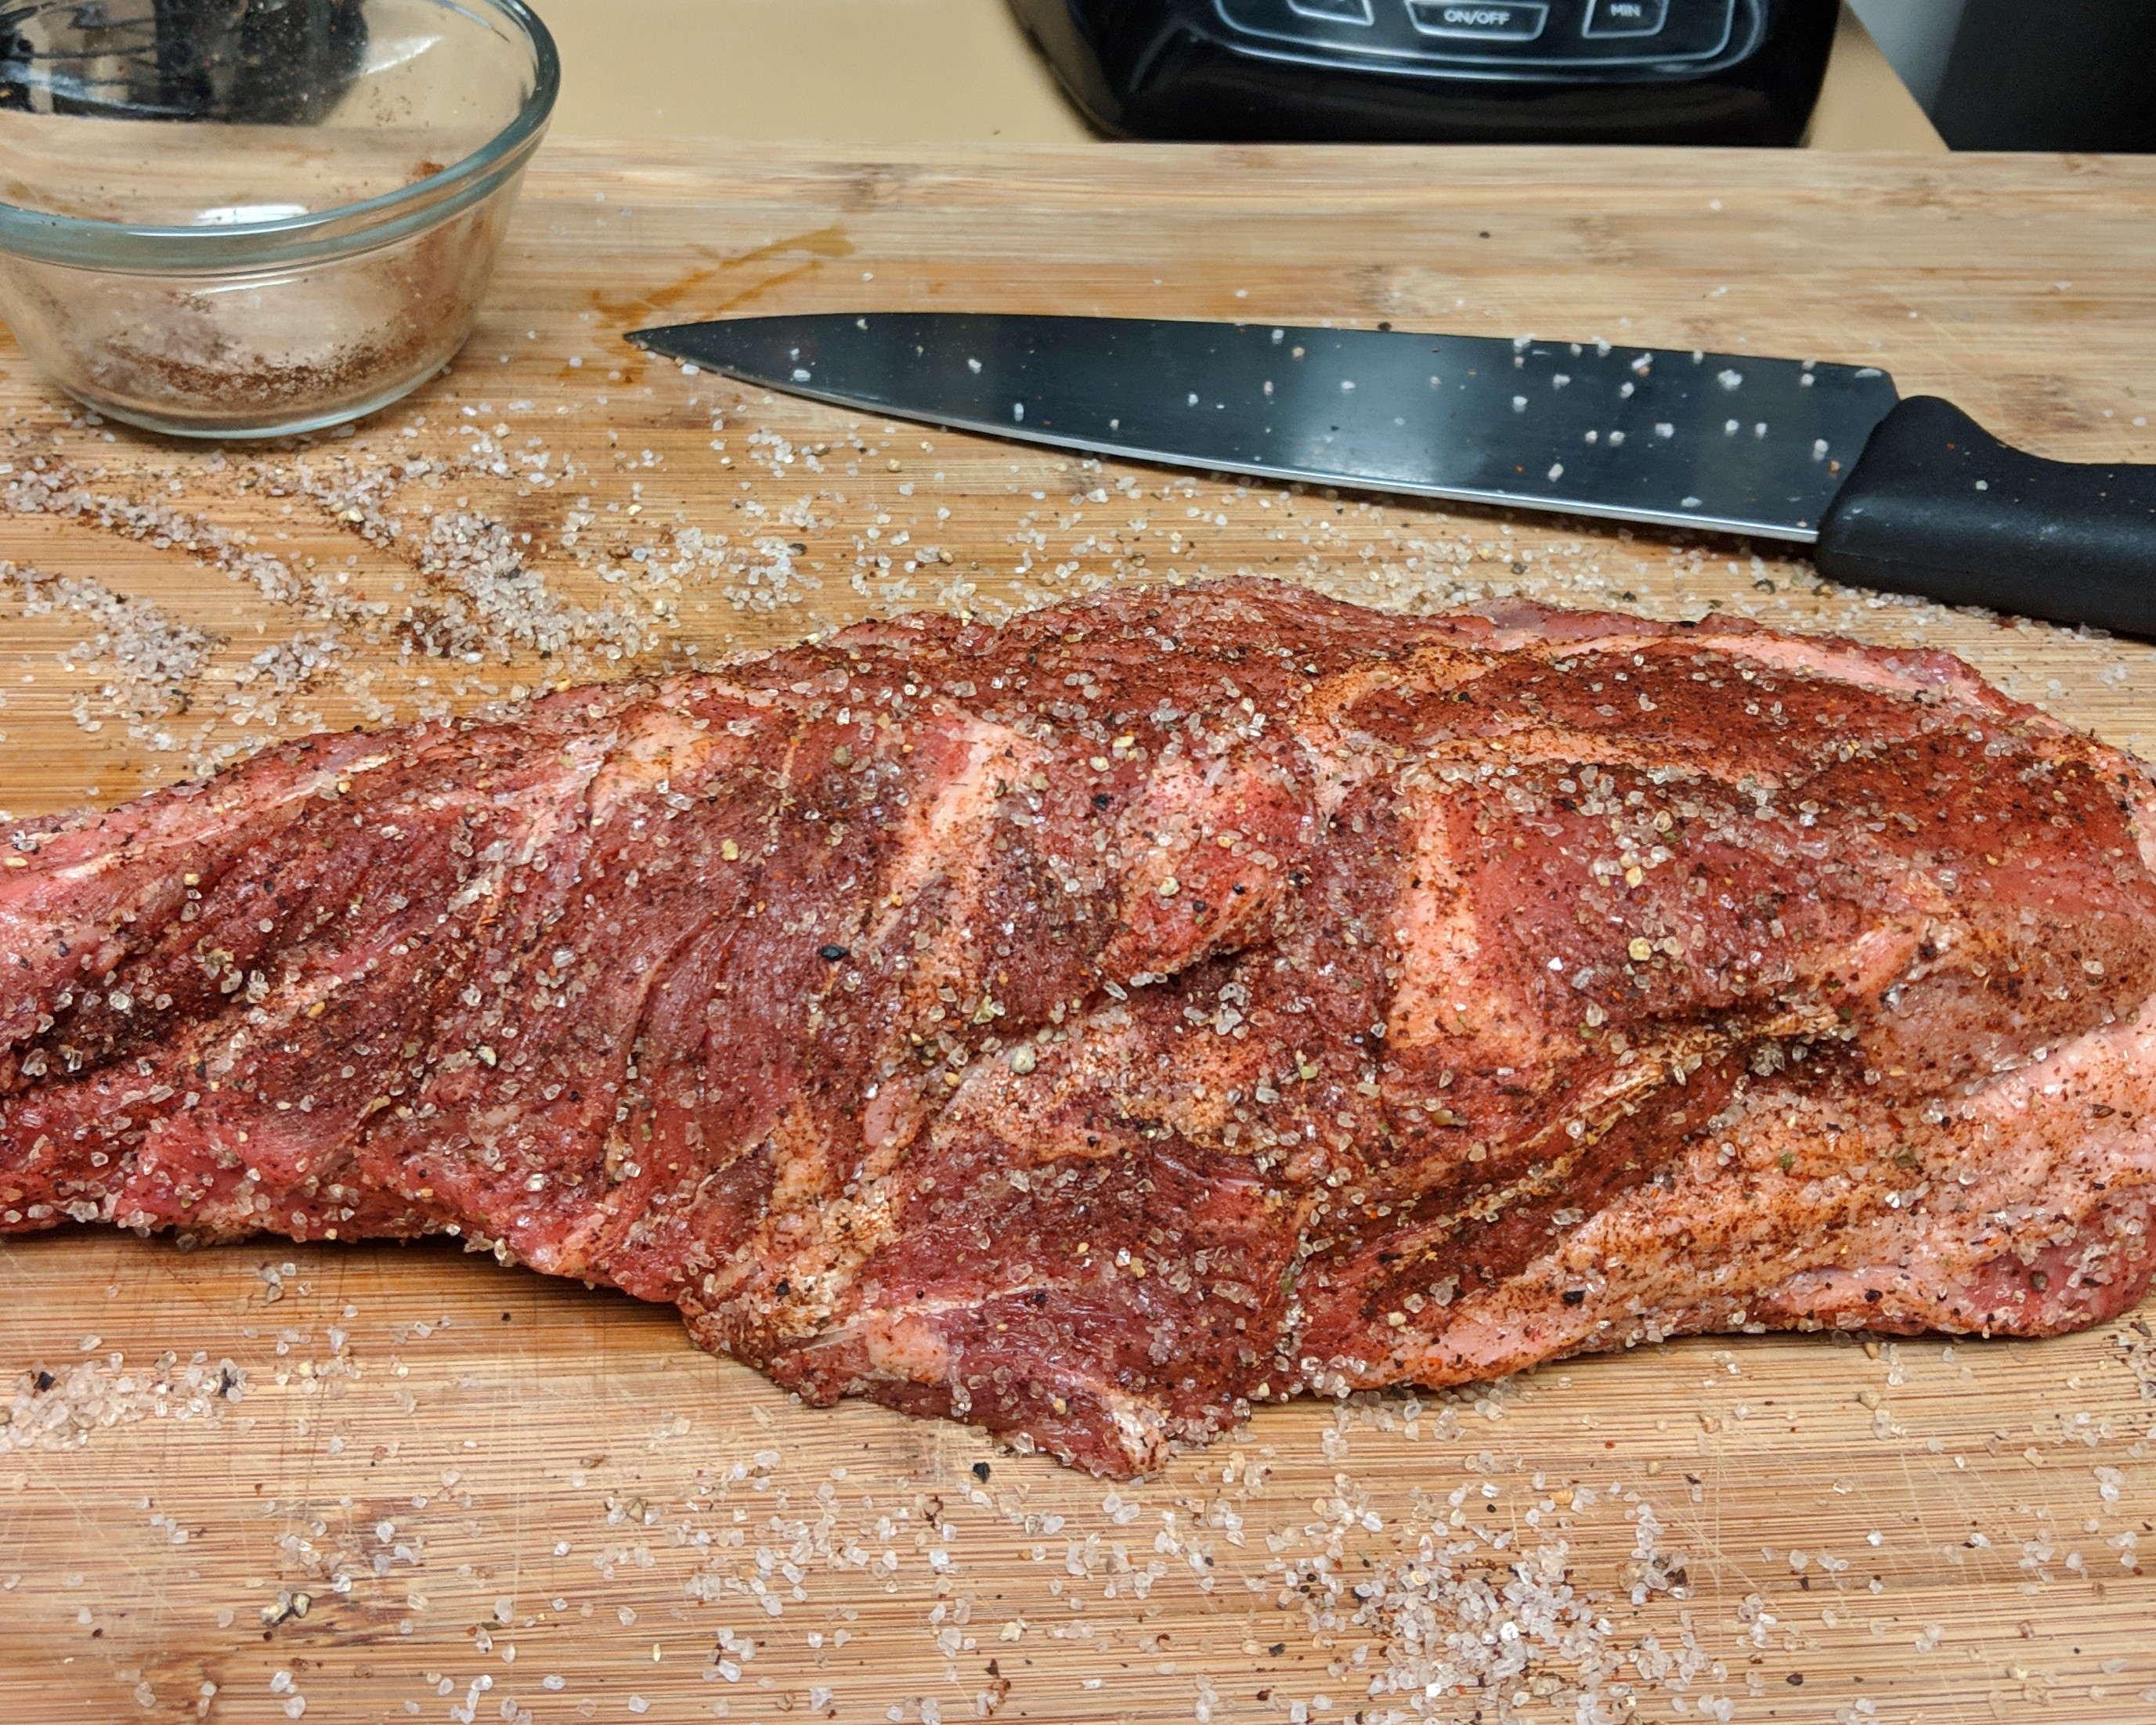
\includegraphics[align=c, height=3in]{recipes/Mexican Shredded Beef/shred_beef.jpg}

\vspace{5 mm} \hrule 

\subsection{Ingredients}\label{ingredients-4}

\begin{tabular}{l|l|l}
\hline
Ingredient & Amount & Unit\\
\hline
Chuck Roast & 2 & lb\\
\hline
Olive Oil & 3 & tbsp\\
\hline
Sweet Onion & 0.5 & whole\\
\hline
Garlic & 4 & cloves\\
\hline
Beef Stock & 4 & cups\\
\hline
Tomato Paste & 1 & tbsp\\
\hline
Bell Pepper & 1 & whole\\
\hline
Jalapeno & 1 & whole\\
\hline
Cumin & 1 & tbsp\\
\hline
Cinammon & 1 & tsp\\
\hline
Bay Leaves & 2 & leaves\\
\hline
Chili Powder & 1 & tbsp\\
\hline
Coarse Salt & to taste & \\
\hline
Black Pepper & to taste & \\
\hline
\end{tabular}

\subsection{Steps}\label{steps-4}

\begin{enumerate}
\def\labelenumi{\arabic{enumi}.}
\item
  Preheat the oven to 275°F
\item
  Heat 2 tbsp olive oil in Dutch oven over medium-high heat. Add diced
  onions and garlic. Lightly brown.
\item
  Generously rub the roast with coarse salt, black pepper, and chili
  powder to create a crust.
\item
  Remove the onions and garlic when browned. Add the remaining 1 tbsp
  olive oil to the Dutch oven. Add the roast and sear for about a minute
  on all sides.
\item
  Remove the roast to the bowl with the onions and garlic. Add 1 cup of
  beef stock to deglaze, gently scraping the bottom with a wooden spoon.
\item
  Return the roast to the Dutch oven and add enough beef broth to cover
  at least half way, about 1 to 2 cups.
\item
  Return the onions and garlic, add the peppers and spices, and cover
  with the lid. Place into the warm oven. It should roast for about an
  hour per pound, or until the meat is fall-apart tender.
\item
  Remove the roast from the Dutch oven to a large bowl. Strain the
  remaining onion, peppers, etc. from the broth and set aside for
  toppings. Heat the remaining broth to a boil and reduce by half.
\item
  Using two forks, pull the beef apart until it is shredded. Once the
  broth has reduced, use a ladle to pour it over the shredded beef until
  the moisture and beef are the right consistency.
\end{enumerate}

\break 

\section{Pot Roast}\label{pot-roast}

\hrule  \vspace{5 mm}

\HUGE Pot
Roast\normalsize \hfill 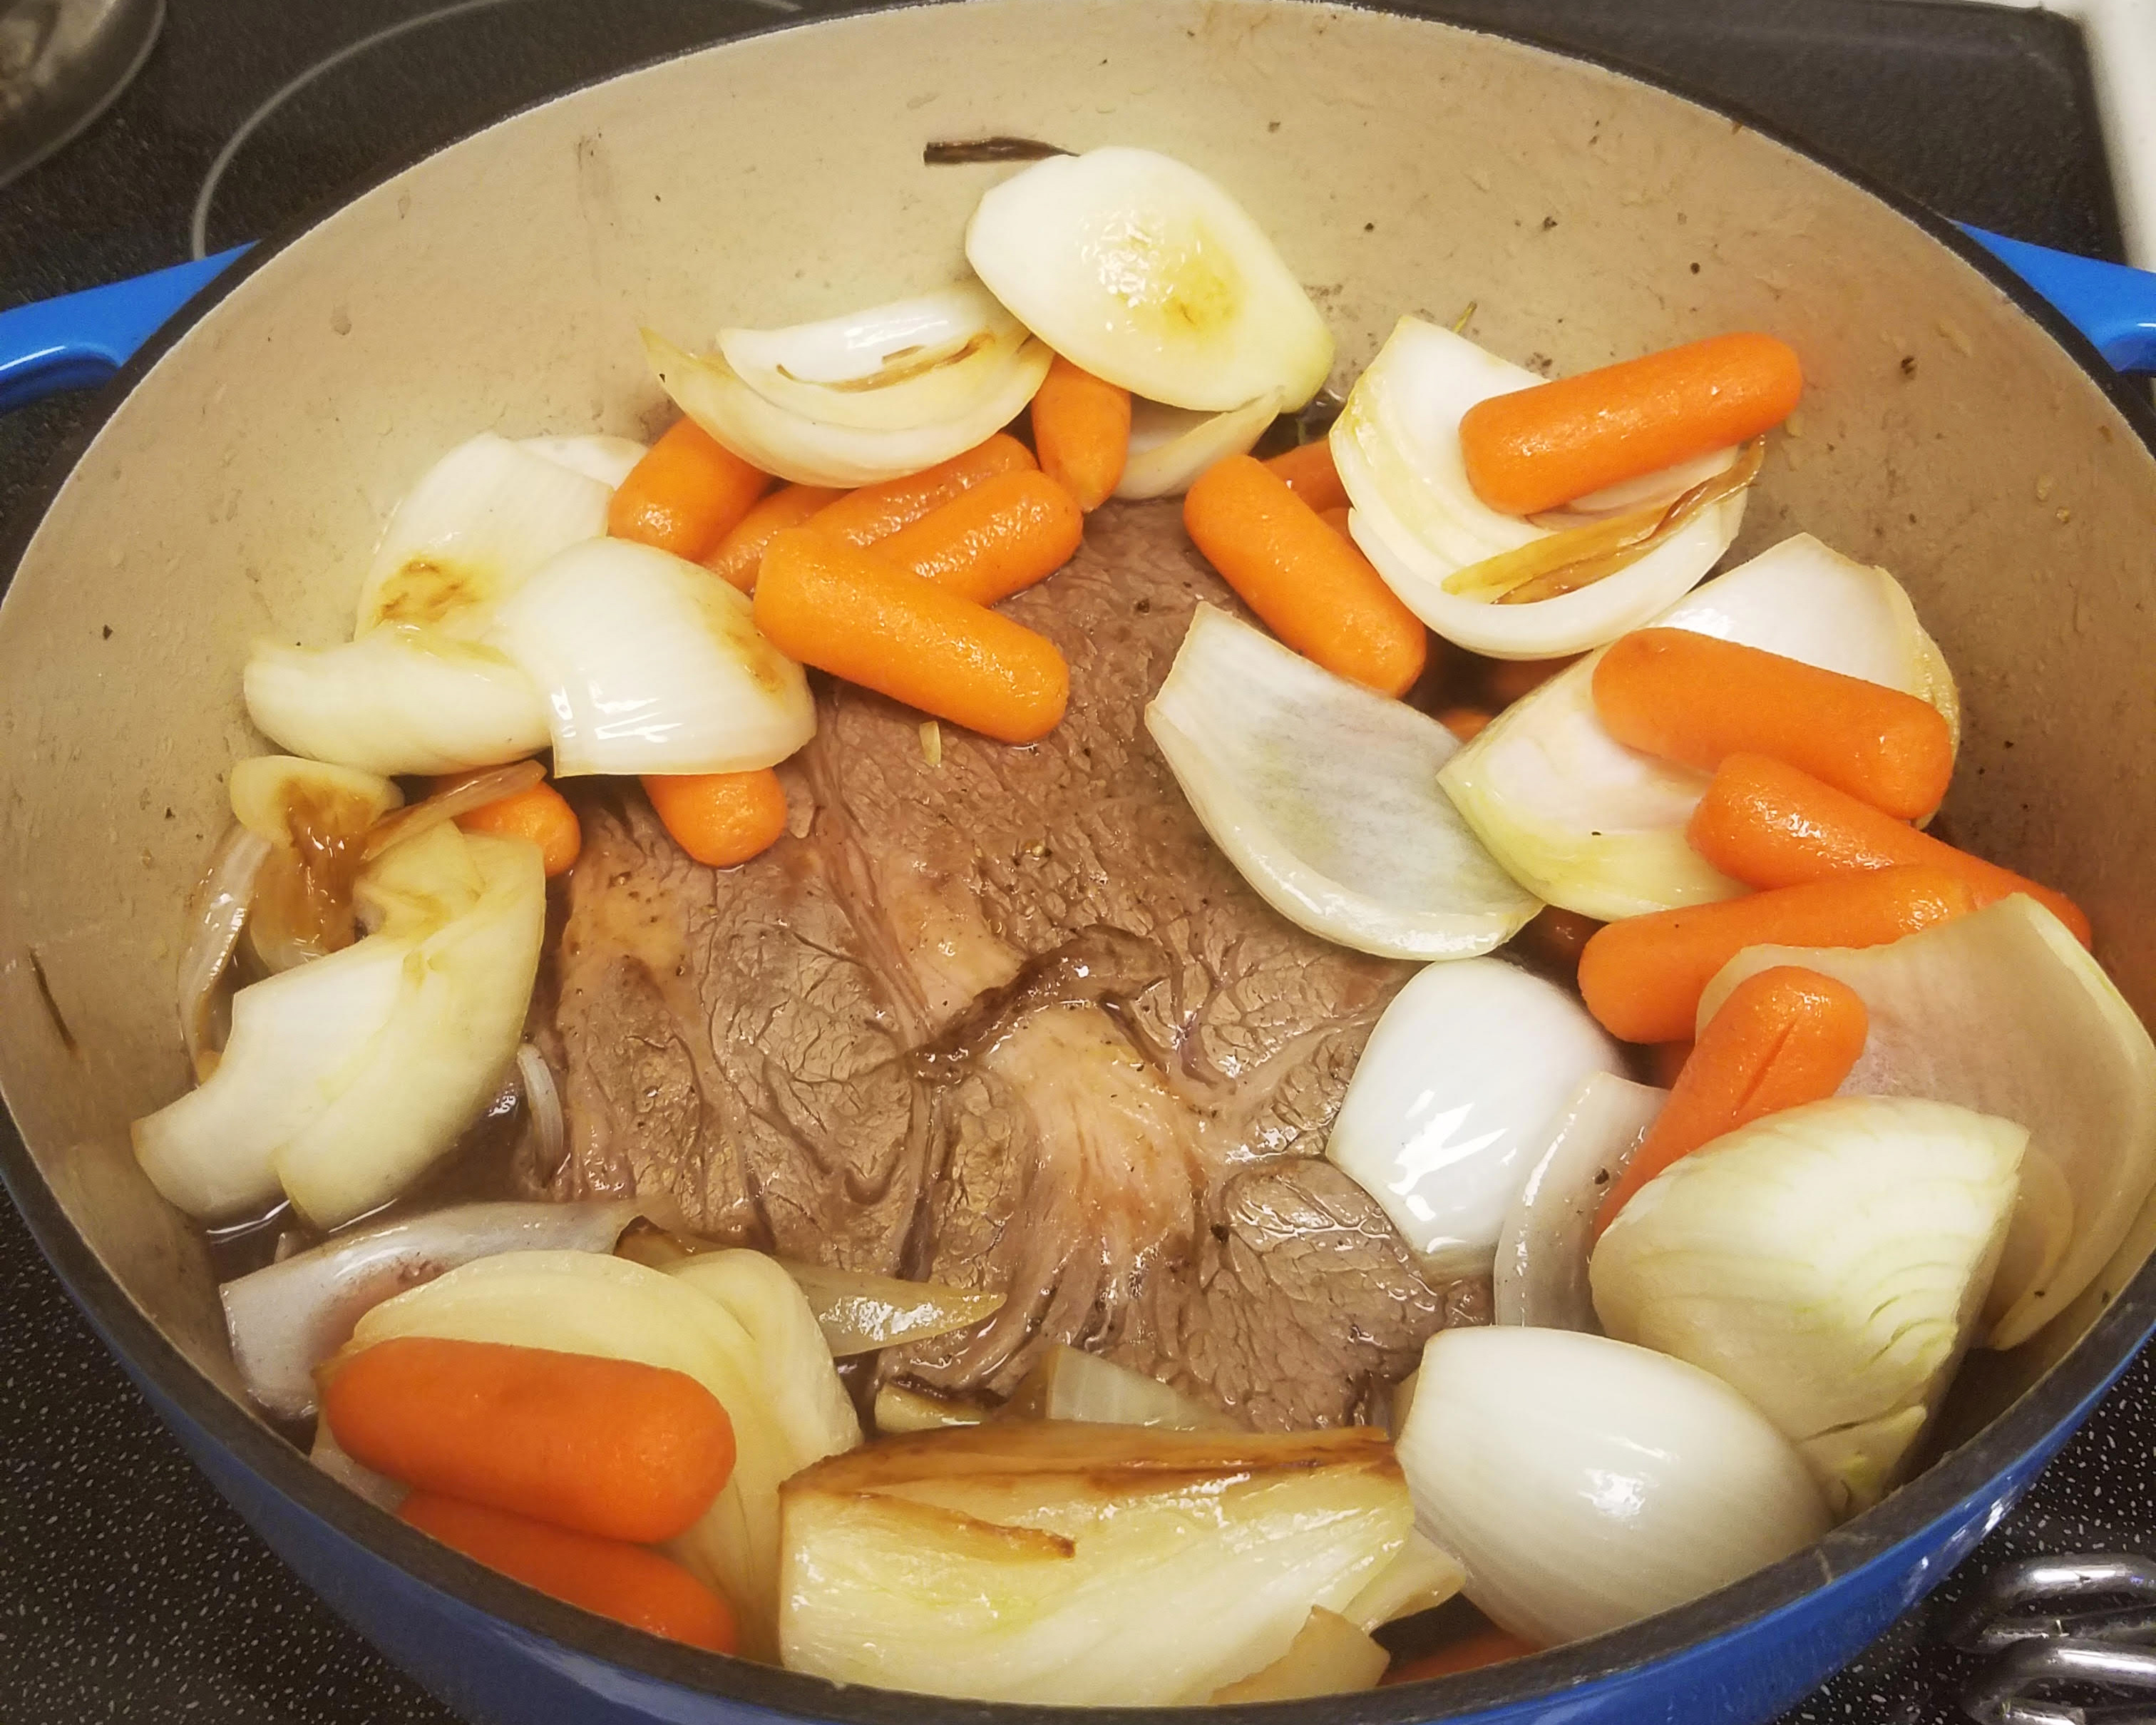
\includegraphics[align=c, height=3in]{recipes/Pot Roast/pot_roast.jpg}

\vspace{5 mm} \hrule 

\subsection{Ingredients}\label{ingredients-5}

\begin{tabular}{l|l|l}
\hline
Ingredient & Amount & Unit\\
\hline
Chuck Roast & 3 to 5 & lb\\
\hline
Olive Oil & 3 & tbsp\\
\hline
Sweet Onion & 2 & whole\\
\hline
Baby Carrots & 1 & lb\\
\hline
Beef Broth & 4 & cups\\
\hline
Red Wine & 1 & cup\\
\hline
Fresh Thyme & 3 to 4 & sprigs\\
\hline
Coarse Salt & to taste & \\
\hline
Black Pepper & to taste & \\
\hline
\end{tabular}

\subsection{Steps}\label{steps-5}

\begin{enumerate}
\def\labelenumi{\arabic{enumi}.}
\item
  Preheat the oven to 275°F
\item
  Heat 2 tbsp olive oil in Dutch oven over medium-high heat. Add
  quartered onions and lightly brown.
\item
  Remove the onions to a large bowl. Add the carrots to the Dutch oven
  and brown.
\item
  Remove the carrots to the bowl with the onions. Add the remaining 1
  tbsp olive oil to the Dutch oven. Add the roast and sear for about a
  minute on all sides.
\item
  Remove the roast to the bowl with the onions and carrots. Add 1 cup of
  red wine to deglaze, gently scraping the bottom with a wooden spoon.
  Let the wine boil for a minute.
\item
  Return the roast to the Dutch oven and add enough beef broth to cover
  at least half way, about 1 to 2 cups.
\item
  Return the onions and carrots, add the fresh thyme, and cover with the
  lid. Place into the warm oven. It should roast for about an hour per
  pound, or until the meat is fall-apart tender.
\item
  Serve over potatoes or with egg noodles.
\end{enumerate}


\end{document}
